\autsection{Descent Vehicle Overall Architecture}{Aaron Gornott}\label{sec:Descent_Vehicle_Overall_Architecture}
The overall design of the lander is influenced by the payload it carries, but a huge design driver is also the chosen descent profile. Since the descent profile itself is driven by the lander design this definition problem circles around itself. As soon as we try to define one part we have to make assumptions about the other. With this in mind the lander design is introduced first to provide a starting reference to the descent profile, but each section will include assumptions that are eventually justified by their framing counterpart.\\
\\
One key aspect of our design is the radiation shielding of our payload. It was decided that the penetrator will be transported vertically with the ground to orbit communication equipment atop. With this approach no mechanism is needed to move both into a fitting orientation when it gets released into a ice hole. By placing the payload in the center of the spacecraft and arranging all other lander components in a symmetric layout around it ensures that the center of mass is at the center of the spacecraft (from a top/bottom view). This provides a solid basis when we have to align the center of the spacecraft with the center of thrust. A tradeoff that follows the decision to orient our payload as a long vertical stick is that top heavy the lander is relative top heavy. The rest of our design choices have to keep this into account.

\subsection{Propellant}
The payload is surrounded by a toroidal fuel tank whose walls also acts as radiation shield. Wall thickness of the inner wall is increased to maximize the material to protection ratio (more info in the radiation section). To counteract the top heavy design fuel tank is conical shaped with a broad basis and a narrow plateau at the top that hosts the communication antenna and a star camera. 
Three types of fuel are used for different purposes and are selected with a focus of long term space storability. Cryogenic propellant like LH + LOX (liquid hydrogen + liquid oxygen) are disqualified, despite their excellent performance, for their quick evaporation and complex temperature demands that increases the risk of tank overpressure. Solid rockets on the other hand are very safe to transport (no fuel sloshing) and provide good storability as well as reliable ignition. Due to the lack of controllability after ignition they are only suitable to address rough delta v changes. We disqualified solid rocket motors as well because they possess a poor specific impulse. The lander need to slow down at least 3.3 km/s  and with a already heavy payload to deliver the fuel is required to have a higher mass to energy density. (Our orbiter + lander total mass constraint in Jupiter orbit is 4.9 tons. Later calculations with higher ISP will show that this mass maximum is already reached and therefore main breaking engines with a ISP less than 300 seconds (solid booster performance) are not a feasible solution.)

\begin{figure}[htb]
	\centering
	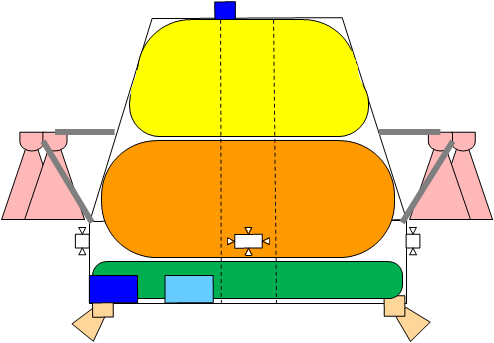
\includegraphics[width=\textwidth]{Lander/aaronfueltank}
	\caption{Fuel tanks side view (height 2m, max width 2m, min width 1.2m, hollow cilinder diameter 30cm): yellow - nitrogen tetroxide (N2O4), orange - unsymmetrical dimethylhydrazine (UDMH), green - High Performance Green Propellant \label{fig:afuelTank}}
\end{figure}

To kill the main delta v two component hypergolic propellant will be used and stored in tiers of fuel tanks on top of each other as shown in figure \ref{fig:afuelTank} Fuel tanks side view. The conservative choice of hydrazine + dinitrogen tetroxide enables the  use of broadly available COTS (Commercial of the Shelf) propulsion components. However propulsion components involved in the final touchdown phase will operate with HPGP mono propellant (High Performance Green Propellant (e.g. LMP-103S)). With HPGP landing site contamination of toxic hydrazine is avoided. Especially the propulsive ice melting gains big benefits from this green propellant, particularly avoiding hydrazine which is extreme deadly for Earth water organisms. The RCS (Reaction control System) operates during touchdown and therefore also has to use HPGP. Luckily HPGP is compatible with most construction materials used in Hydrazine COTS components and propulsion systems. In the final phase before touchdown the bipropellant tanks are expected to be empty, to increase stability at surface contact the green propellant fuel tanks will be located at the bottom of the lander to keep a low the center of mass.\\
Delivering propellant from the tanks to the thrusters in microgravity comes not for free and needs a technical system. Due to the complex conical and toroidal tank shape piston or inflatable bladders will not be practicable. A diaphragm is very adaptable to non trivial shapes and will push the propellant through pipe outlets and opened propellant valves. Helium containing spheres  are responsible to apply pressure on the empty site of the fuel tank diaphragm. It is necessary to regulate tank pressure with a helium valve system.\\

\subsection{Propulsion System}
The lander features three distinctive rocket motor systems with unique rolls: 1 - main breaking engine, 2 - touchdown engine, 3 - RCS (see RCS section \ref{XXX}).

\begin{figure}[htb]
	\centering
	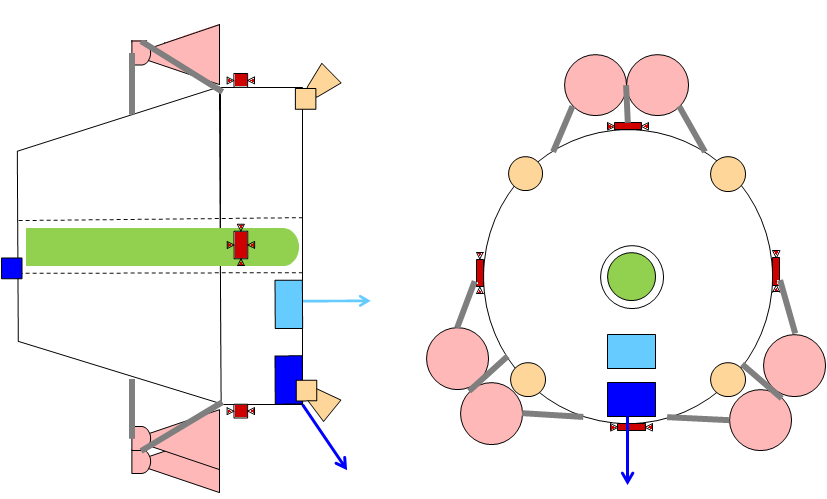
\includegraphics[width=\textwidth]{Lander/aaronlanderprop}
	\caption{Propulsion system (left - side view, right - bottom view): light red - main breaking engine, light orange - touchdown engine, dark red - RCS, light green - ice penetrator, dark blue - navigation instruments for main descent phase (arrow indicates sensor direction that avoids main breaking engine exhaust plume), light blue - navigation instruments for touchdown (arrow indicates sensor direction that avoids touchdown engine exhaust plume)\label{fig:alanderprop}}
\end{figure}

\subsubsection{Bain Breaking Engine} 
Overall intended thrust for the main braking is 25 kN. The chosen design features three scaffolds outstretching from the spacecraft with each scaffold has two rocket motors attached. Close to the predefined performance of 4.17 kN is the KRD-442 \cite{AstronauticaKRD} N2O4/UDMH rocket engine with 4.38 kN, currently flying on the international space station module Zarya. A KRD-442 weights 52kg and we need six units, this is way beyond our propulsion mass limit, but it is realistic to develop a similar engine with only half of the mass by relinquishing unnecessary features and using modern production techniques as well as materials. For instance the KRD-442 can throttle down to extreme low 0.17 kN, we do not need such a flexible design.\\
The main propulsion system architecture is a result of practical consideration laid out in the following. To create maximum stability during the breaking burn we choose not to place the breaking engine at the bottom where high precision balancing of the top-heavy spacecraft is necessary. Instead the breaking force should be applied from a point of attack higher than the center of mass to enable the whole system to balance itself. For weight saving and complexity reduction all thruster are fix attached to the structure scaffold without any gimbal mechanism. Select a three armed scaffold structure resulted from the need of a two axis rotation redundancy. Assuming all thrusters are orientated in the same direction, with one fixed thruster no rotation in possible through thrust modification. Two fixed thrusters allow for one axis of rotation, and three or more allow for two axis rotation. Not choosing more than three arms minimizes structure overhead that would accrue without additional benefit, moreover dividing the same thrust among more thrusters also worsens the mass to thrust ratio. Finally the split of two rocket engines per arm is another level of redundancy as well as a aspect of the commercial availability in the needed thrust range. For redundancy it is to consider that if a main engine fails two at the other arms has to be shut down as well for balancing purposes. This gives a theoretical failure tolerance of three main engines. Of course any initial intended landing profile will no longer be executable with only 50\% of the expected thrust, but with high enough fuel and radiation shielding margins that can exceed time and delta v requirements new emergency possibilities can become possible. Similar to the recently saved Akatsuki \cite{AkatsukiRescue} probe whose Venus orbit insertion thrusters failed to fire in 2010 but orbit insertion was achieved in 2015 only with its attitude control thrusters.\\

\subsubsection{Touchdown Engine} 
Reducing the horrizontal delta v required high thrust, whereas in the the final descent phase before touchdown propulsion requirements change. For this reason our descent vehicle has it own engines for this final phase. The new minimal thurst requirement have to provide enought force to enable hoover manuvers to avoid late detected ground hazzards. Needed thrust can be calculated by multipliing the lander mass with its gravitation environment. Additionaly to this minimum value other facotrs has to be accounted for. As stated before to prevent landing site contamination HPGP is used for the touchdown engines. Their exhaust becomes a danger for the lander and the payload when pointed straight to the ground, if recoiling ground particles hit sensible components. Another problem with ground faceing engines during touchdown is that the Navigation instruments have to operate though the exhaust plume. Depending on the instruments this can lower the data qualitiy or prevent operation at all. To avoid or minimise this issuees the touchdown engines are angles 22.5° this reduces the efective fuel use by 25\%. Atop of this loss there is the lower ISP caused by the propellant this means there is a high incentive to use the main breaking engine as long as possible. To have any matematical justification for the handover time that swtiches to the touchdown engine the horrizontal and vertical velocity is split and after the equivalent of horrizontal v is slowed down the engine handover occurs. The notion "equivalent of horrizontal" means that also some of this thrust during the gravity turn is used vertivaly. In theory this becomes important in staged descent profiles that a small remaining horizontal v ensures the contamined rocket mortors do not crash where the lander intens to land, right under the lander (This is only not relevant for the choosen lander design, in the landing profile section we argument why we do not use staging).\\
The touchdown engines are attached to the bottom fuel tank structure this is the widest point of the lander (exept landing legs and main engine scaffold arms). Low attachment makes sense because the HPGP tank is also at the bottom. Whereas the N2O4/UDMH tanks are emtey and therefore the center of mass has shifted to the bottom.Four engines will be used, recall that three are necesarry for two axis controll plus the fouth to increse manuvrebility. Increasing thrust points adds up more flexibility on executing manuveres within the engine configuration. Rough manuvres can by executed with thrust throtteling again there is no additional gimbal mechansim. Fine manuveres are executes by the RCS\\
Based on the initial minimal thrust reqirement with all constrains combined it can expeted that roughly double the performance is needed (margin). The following calculation used the lander wet-mass after the main breaking engine stops firering.
$$2 * 1102 kg * 1.315 m/s^2 = 2898 N = 4 * 725 N$$
Currently there is no 725 N HPGP engine available, but it is possible to develop one. The hydrazine engine LEROS 1b in the same thrust class (635 N, 4.5kg) can give us a good reference about the expected weight of roughly 5kg.


\subsection{Landing Legs}
Landing legs provide a stable structure for the touchdown, some also absorb the final impact with a suspension mechanism. A short look to into the history shows that a wide spectrum designs were successfully applied.\\
 Luna 9 was the first probe that landed 1966 on another celestial body. Its minimalistic method was not having a landing structure at all. Instead the descent vehicle approached the surface for a soft touchdown but 5 m above the surface the payload got catapulted a safe distance away before the descent stage crashes or at least tips over. This method was chosen by the soviets because it simplifies the moment of surface contact, when the most precision is needed for a soft landing. There are a couple of reasons why this method will not be suitable for our straw man. Most importantly the orientation of our payload matters and randomly ejecting it away will make it hard to point the penetrator with it RTG downwards. Secondly the propulsive ice melting is logically be executed from the descent vehicle, since it already has fuel tanks to hold everything in place and propulsive components to support the needed thrusters.  Another big argument against sacrificing the descent vehicle is it provides structure that provides additional radiation shielding and serves as communication relay station between the ice penetrator and the orbiter.\\
\\
A similar minimalistic approach in not having classical landing legs is simply landing on the vehicles structure. Google Lunar XPRIZE team Moon Express utilizes such a landing platform that is intended to land on in tank structure with an energy absorbing material at its bottom. Not having outstretching legs safes weight and space, but increases the overall risk of tipping over unless the design is not flat and wide (This limits the possible vehicle architectures). Despite these limitation the critical argument against landing on the core structure (or even worse: airbags) is that the propulsive ice melting needs free space for the rocket exhaust and should also avoid accumulating refreezing ice on sensitive vehicle components (like the penetrator release mechanism).\\
\\
Outstretching landing legs allow to build taller lander architectures. Most comely are four or three legged designs. The four legged Luna 16 probe or the three legged Surveyor moon probes are a good example for this height to diameter ratio. Surveyors height was 3 m and its footpads extended out 4.3 m. More legs means more stability, therefore design with less legs need increased leg length (and strength) to compare in stability. This implies if you add additional legs you not necessarily add more weight. However longer legs are beneficial by increasing the distance to the exhaust of the propulsive melting. \\
A three legged design is chosen as suitable lander design for our Europa lander. The three legs itself consisting out of three rods similar to the Luna 16 design. Two rods will spread toward the lower end of the lander and the third one is attached at a higher point. The legs will stretch out 1.3 meter from the spacecrafts fuel tank (2 meter diameter).  Launched under the 5 m Atlas V fairing there is no need for a fold up mechanism.\\
\\
JPL proposed a six legged vehicle in its Europa Lander 2012 Report that features a very useful footpad design. They call it "skid \& tip over mitigation feet" the food is lengthened by a curved tongue that can reduce the tip over risk and adjust the vehicles orientation. We chose to adapt the curved tongue part of the feet that can slide on the ice in case of a suboptimal touchdown, but do not adapt the skid part at the bottom site. Instead of the bottom skid we have some ice spikes cause we have to prevent post landing movement under all circumstances (losing the penetrator/communication hole). Harsh breaking by spikes increases the tip over risk but the tip over mitigation tongue is a useful countermeasure.

\begin{figure}[htb]
	\centering
	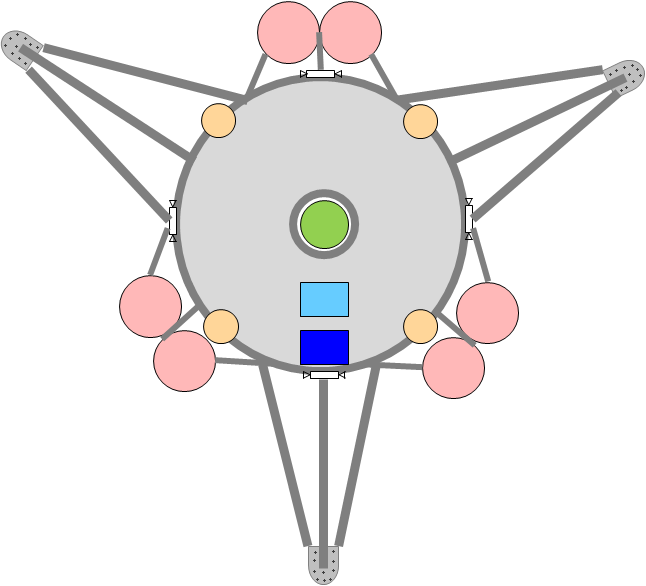
\includegraphics[width=\textwidth]{Lander/aaronlandinglegs}
	\caption{Landings legs (bottom view): dark grey - structure scaffold \label{fig:alanderlegs}}
\end{figure}

\subsection{Mechanisms}
..


\subsubsection{Probe Release Mechanism}
...

and orbiter adpter
...

\subsubsection{Ice Communication Boom}
...

\subsubsection{Launch Vehicle Adapter}
...

\subsection{Mass Allocation}
The mass allocation for our proposed lander
\\
TOTAL MASS (on the surface) 1000 kg:
\begin{itemize}  
\item Payload (Surface module + ice-descent vehicle + power) 180 kg
\item Navigation 10 kg
\item Propulsion 200 kg
\item Weight of fuel tank + shielding 100 kg
\item Structure 210 kg
\item Landings legs 75 kg
\item Mechanism 25 kg
\item Ice melting propellant 150 kg
\item Margin 50kg
\end{itemize}




\subsection{Landing Profile Analyses}


By numerically analyzing different landing profiles we can compare fuel requirements and 


bruning fuel
suspension mechanism

comunication to penetrator mechanism   



thruster parameters position strength, angle fuel


input parameter:
\begin{itemize} 
\item initial eliptical orbit perigee hight = 100 km
\item initial eliptical orbit perigee velocity = 3.3 km/s
\item orbit direction syncron with Europa rotation = true
\item intendet parking orbit hight = 10 km
\item main breaking engine ISP: 310 s
\item touchdown engine ISP = 234 s
\item effective useable thrust for touchdown burn = 75\%
\end{itemize}


profile 5\\
Staged Mass  - 60 kg\\
Staging Mechanism + 10 kg\\
\\
profile 3 and 6\\
Staged Mass  - 40 kg\\
"Staging Mechanism" + 5 kg \\
"only one engine savings" - 20 kg



\begin{figure}[htb]
	\centering
	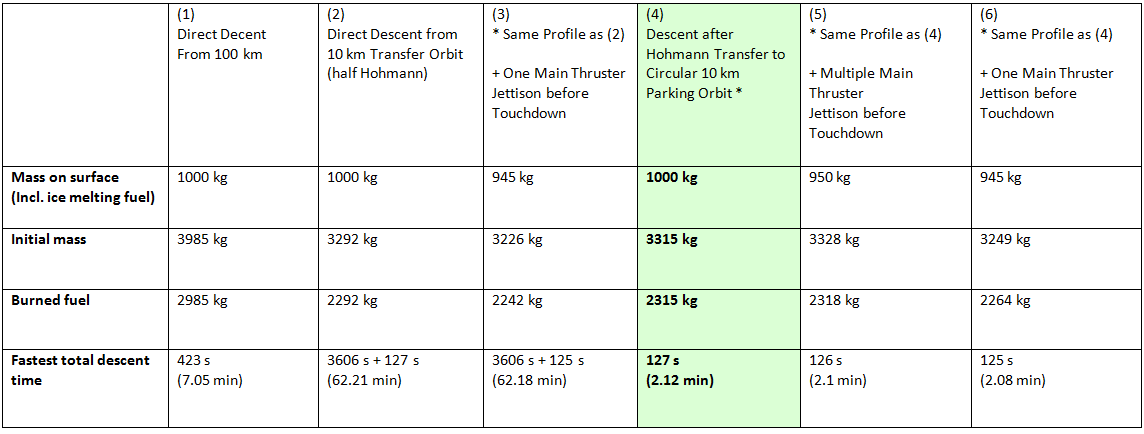
\includegraphics[width=\textwidth]{Lander/aaroncomparison}
	\caption{Landing profile comparison\label{fig:acomparison}}
\end{figure}


\begin{figure}[htb]
	\centering
	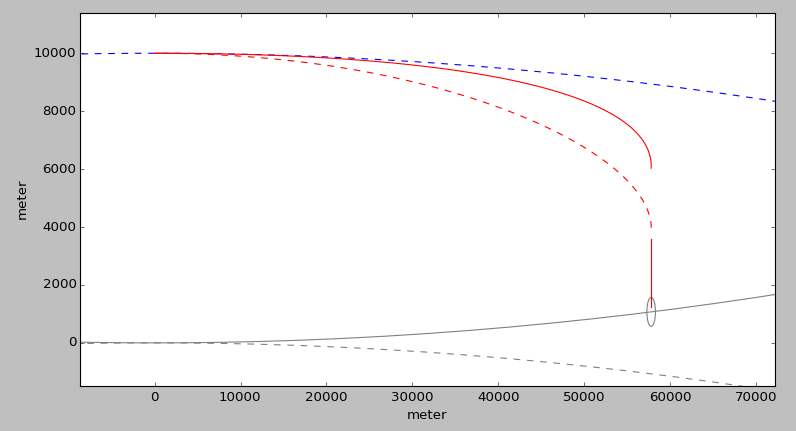
\includegraphics[width=\textwidth]{Lander/aaronlandingprofile}
	\caption{Selected landing profile (4)\label{fig:alandingprofile}}
\end{figure}



\begin{lstlisting}[caption={Simulation details from profile (4)}, label=acalcoutput]
=== Calculation Results ===

> initial burn at perigee (100.0 km) to
> transform elliptical orbit into circular orbit

   circular orbit velocity: 1388.30270225 m/s
   circular orbit period: 7516.45454646 s (125.274242441 min)

   delta v: 1911.69729775 m/s

> Hohmann transfer to 10.0 km
   dv1: 19.4686094861 m/s
   dv2: 20.018574823 m/s
   transfer duration: 3606.52080051 s (60.1086800085 min)

   circular orbit velocity: 1427.52062194 m/s
   circular orbit period: 6913.82480145 s (115.230413358 min)

   burned fuel so far: 1570.8654837 kg
   burn duration so far: 190.891573579 s (3.18152622632 min)

> descent burn to kill horizontal velocity: 1395.55813424 m/s

   burned fuel: 642.312338423 kg
   horizontal burn time: 79 s (1.31666666667 min)

> tilt over window: 24.5463652703 s

> final touchdown burn

   accumulated gravity delta v: 166.336001329 m/s
   burned fuel: 101.548930606 kg
   burn duration: 16.4536347297 s (0.274227245495 min)

> total DESCENT time: 127.144607321 s (2.11907678868 min)

> TOTAL fuel burned by lander: 2314.72675273 kg
> LANDED semi dry mass (lander + fuel margin left): 1000.05106939 kg
\end{lstlisting}


\begin{itemize}  
\item 860 kg (descent vehicle dry mass)
\item + 2318 kg (optimal landing profile propellant)
\item + 126 kg (7\% propellant for RCS) = 2480 kg
\item + 496 kg (20\% overall margin) =  2976 kg 
\item + 150 kg (ice melting propellant)
\item = 3986 kg (TOTAL)
\end{itemize}  

Dry mass

landing profile
overall design with weights 
	
	structure
	material
	landing legs
thermal environment


\subsection{Descent Validation}

Validation by comparison 

proofing claims
	lander design by comparison
	descent profile by analysis


Target gravity: Europa 1,315 m/s²

List of all bodies where S/C performed a controlled landing (to prove valid design)

Landings with atmosphere a.k.a. cheating the  delta v away:
\begin{itemize}  
\item Venus 8,87 m/s²
\item Mars 3,711 m/s²
\item Titan 1,352 m/s²
\end{itemize}

Pure propulsion landings:
\begin{itemize}
\item Moon 1,622 m/s²
\item 433-Eros 0.0059 m/s² (asteriod landing with highest gravity so far)
\item Phobos 0,0057 m/s² (3 failed probes)
\item Churyumov–Gerasimenko ~0.001 m/s²
\item 25143-Itokawa ~0.0001 m/s² (sample return)
\end{itemize}
